\documentclass{article}
\usepackage{graphicx}
\usepackage{amsmath}
\usepackage{booktabs}
\usepackage{siunitx}
\usepackage{float}
\usepackage{listings}
\usepackage{xcolor}

\lstset{
  language=Matlab,
  basicstyle=\ttfamily\small,
  keywordstyle=\color{blue},
  commentstyle=\color{green!50!black},
  stringstyle=\color{red!70!black},
  frame=single,
  breaklines=true
}

\title{Homework Assignment 2 \\ \large Analogue Integrated Circuit Design --- ET4252}
\author{
  Raghavendra Joshi \\ Student Number: 6438180 \\
  \and
  Daniel Tyukov \\ Student Number: 5714699 \\
  \and
  \textit{Microelectronics, TU Delft}
}
\date{March 2026}

\begin{document}

\maketitle

\section*{Objective}
The purpose of this problem is to confirm the inapplicability of the square-law formula for the \SI{180}{nm} MOS devices in the ET4252 technology. Finite output resistance is neglected in all calculations.

\tableofcontents
\newpage

%% ====================================================================
\section{Part A: Operating Point Simulation}
%% ====================================================================

Use an operating point simulation (\texttt{.op}) to measure the drain current of an NMOS transistor with $W/L = \SI{5}{\micro m}\,/\,\SI{0.18}{\micro m}$ at $V_{DS} = \SI{1.5}{V}$ and $V_{GS} = \SI{0.6}{V}$ and $\SI{1.5}{V}$.

\subsection{Circuit}

\begin{figure}[H]
\centering
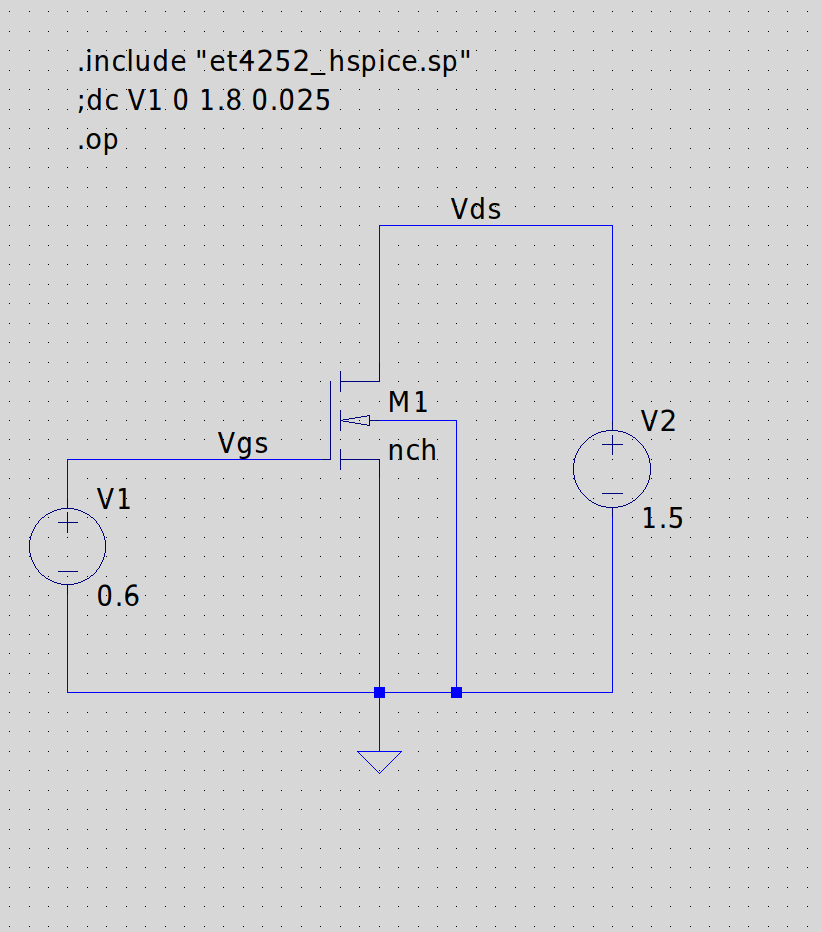
\includegraphics[width=0.65\textwidth]{imgs/partA_schematic.png}
\caption{LTSpice schematic: NMOS M1 (\texttt{nch} model, BSIM3v3, \SI{180}{nm}), $W/L = \SI{5}{\micro m}\,/\,\SI{0.18}{\micro m}$. $V_{DS} = \SI{1.5}{V}$ provided by V2, $V_{GS}$ set by V1. Bulk tied to source (ground).}
\label{fig:partA_schematic}
\end{figure}

\subsection{Operating Point Results}

\begin{table}[H]
\centering
\caption{Simulated drain current at the two operating points.}
\label{tab:partA}
\begin{tabular}{@{}ccc@{}}
\toprule
$V_{GS}$ & $V_{DS}$ & $I_D$ \\
\midrule
\SI{0.6}{V} & \SI{1.5}{V} & \SI{79.26}{\micro A} \\
\SI{1.5}{V} & \SI{1.5}{V} & \SI{2.284}{mA} \\
\bottomrule
\end{tabular}
\end{table}

\begin{figure}[H]
\centering
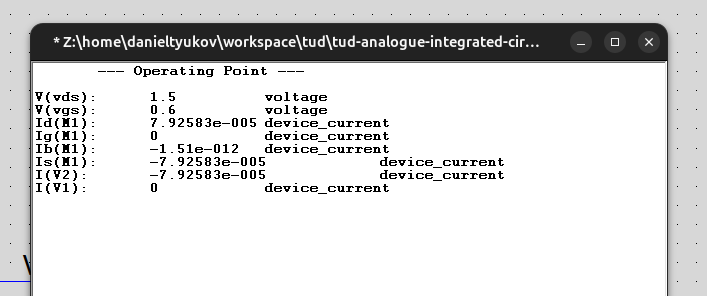
\includegraphics[width=0.75\textwidth]{imgs/partA_op_vgs0.6V.png}
\caption{Operating point results at $V_{GS} = \SI{0.6}{V}$, $V_{DS} = \SI{1.5}{V}$: $I_D = \SI{79.26}{\micro A}$.}
\label{fig:partA_op06}
\end{figure}

\begin{figure}[H]
\centering
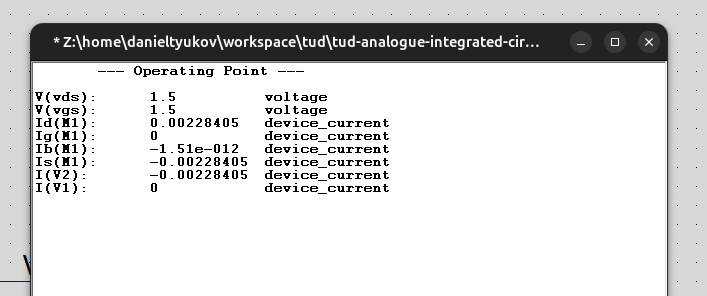
\includegraphics[width=0.75\textwidth]{imgs/partA_op_vgs1.5V.png}
\caption{Operating point results at $V_{GS} = \SI{1.5}{V}$, $V_{DS} = \SI{1.5}{V}$: $I_D = \SI{2.284}{mA}$.}
\label{fig:partA_op15}
\end{figure}

%% ====================================================================
\section{Part B: Extracting $V_t$ and $\mu_n C_{ox}(W/L)$}
%% ====================================================================

Using the data from part~(a), we estimate the threshold voltage $V_t$ and $\mu_n C_{ox}(W/L)$ assuming the square-law model.

\subsection{Method}

The square-law model in saturation (neglecting finite output resistance):

\begin{equation}\label{eq:squarelaw}
I_D = \frac{1}{2}\,\mu_n C_{ox}\,\frac{W}{L}\,(V_{GS} - V_t)^2
\end{equation}

Let $K = \frac{1}{2}\,\mu_n C_{ox}\,\frac{W}{L}$. From the two simulated data points:

\begin{align}
I_{D1} &= K\,(V_{GS1} - V_t)^2 \quad \Rightarrow \quad 7.92583 \times 10^{-5} = K\,(0.6 - V_t)^2 \label{eq:id1} \\
I_{D2} &= K\,(V_{GS2} - V_t)^2 \quad \Rightarrow \quad 2.28405 \times 10^{-3} = K\,(1.5 - V_t)^2 \label{eq:id2}
\end{align}

Dividing~\eqref{eq:id2} by~\eqref{eq:id1} eliminates $K$:

\begin{equation}
\frac{I_{D2}}{I_{D1}} = \frac{(V_{GS2} - V_t)^2}{(V_{GS1} - V_t)^2}
\end{equation}

\subsection{Solving for $V_t$}

\begin{equation}
r = \sqrt{\frac{I_{D2}}{I_{D1}}} = \sqrt{28.818} = 5.368
\end{equation}

\begin{equation}
r\,(V_{GS1} - V_t) = V_{GS2} - V_t
\end{equation}

\begin{equation}\label{eq:vt}
V_t = \frac{r \cdot V_{GS1} - V_{GS2}}{r - 1} = \frac{5.368 \times 0.6 - 1.5}{5.368 - 1} = \SI{0.394}{V}
\end{equation}

\subsection{Solving for $\mu_n C_{ox}(W/L)$}

\begin{equation}
K = \frac{I_{D1}}{(V_{GS1} - V_t)^2} = \frac{7.92583 \times 10^{-5}}{(0.206)^2} = 1.868 \times 10^{-3}\,\si{A/V^2}
\end{equation}

\begin{equation}\label{eq:mucox_wl}
\mu_n C_{ox}\frac{W}{L} = 2K = 3.736 \times 10^{-3}\,\si{A/V^2} = \SI{3.736}{mA/V^2}
\end{equation}

Extracting $\mu_n C_{ox}$ alone ($W/L = 5/0.18 = 27.78$):

\begin{equation}\label{eq:mucox}
\mu_n C_{ox} = \frac{3.736 \times 10^{-3}}{27.78} = \SI{134.5}{\micro A/V^2}
\end{equation}

\subsection{Summary}

\begin{table}[H]
\centering
\caption{Extracted square-law parameters from the two operating points.}
\label{tab:partB}
\begin{tabular}{@{}ll@{}}
\toprule
Parameter & Extracted Value \\
\midrule
$V_t$ & \SI{0.394}{V} \\
$\mu_n C_{ox}(W/L)$ & \SI{3.736}{mA/V^2} \\
$\mu_n C_{ox}$ & \SI{134.5}{\micro A/V^2} \\
\bottomrule
\end{tabular}
\end{table}

%% ====================================================================
\section{Part C: Square-Law vs.\ Simulation}
%% ====================================================================

Using the results from part~(b), calculate the drain current and transconductance of an NMOS with $W/L = \SI{20}{\micro m}\,/\,\SI{0.7}{\micro m}$ at $V_{DS} = \SI{1.5}{V}$ and $V_{GS} = \SI{0.75}{V}$ using the square-law formula. Then compare against LTSpice simulation.

\subsection{Square-Law Prediction}

Using extracted parameters from part~(b): $V_t = \SI{0.394}{V}$, $\mu_n C_{ox} = \SI{134.5}{\micro A/V^2}$. New aspect ratio: $W/L = 20/0.7 = 28.571$.

\textbf{Drain current:}

\begin{equation}
I_D = \frac{1}{2}\,\mu_n C_{ox}\,\frac{W}{L}\,(V_{GS} - V_t)^2 = \frac{1}{2} \times 134.5 \times 10^{-6} \times 28.571 \times (0.75 - 0.394)^2
\end{equation}

\begin{equation}\label{eq:id_squarelaw}
I_D = 1.922 \times 10^{-3} \times (0.356)^2 = 1.922 \times 10^{-3} \times 0.1267 = \SI{243.6}{\micro A}
\end{equation}

\textbf{Transconductance:}

\begin{equation}\label{eq:gm_squarelaw}
g_m = \mu_n C_{ox}\,\frac{W}{L}\,(V_{GS} - V_t) = 134.5 \times 10^{-6} \times 28.571 \times 0.356 = \SI{1.368}{mS}
\end{equation}

\subsection{LTSpice Simulation}

Same circuit as part~(a), with M1 changed to $W/L = \SI{20}{\micro m}\,/\,\SI{0.7}{\micro m}$, $V_{GS} = \SI{0.75}{V}$, $V_{DS} = \SI{1.5}{V}$.

\begin{figure}[H]
\centering
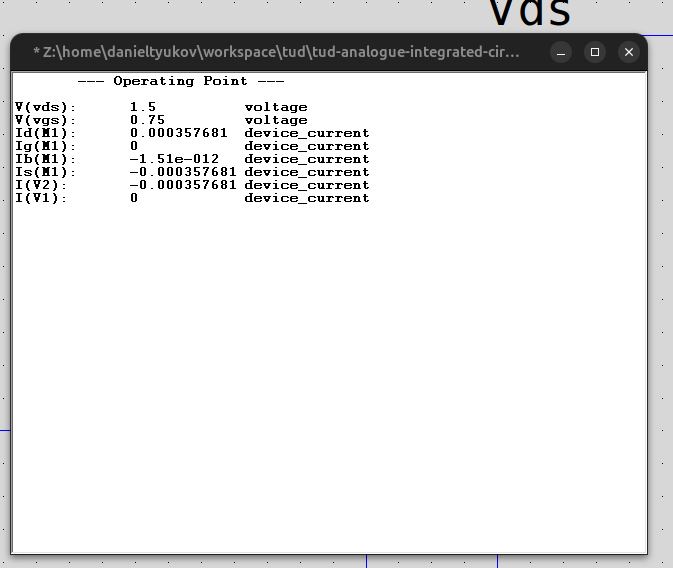
\includegraphics[width=0.75\textwidth]{imgs/partC_op_vgs0.75V.png}
\caption{Operating point results for $W/L = \SI{20}{\micro m}\,/\,\SI{0.7}{\micro m}$ at $V_{GS} = \SI{0.75}{V}$: $I_D = \SI{357.7}{\micro A}$.}
\label{fig:partC_op}
\end{figure}

\begin{figure}[H]
\centering
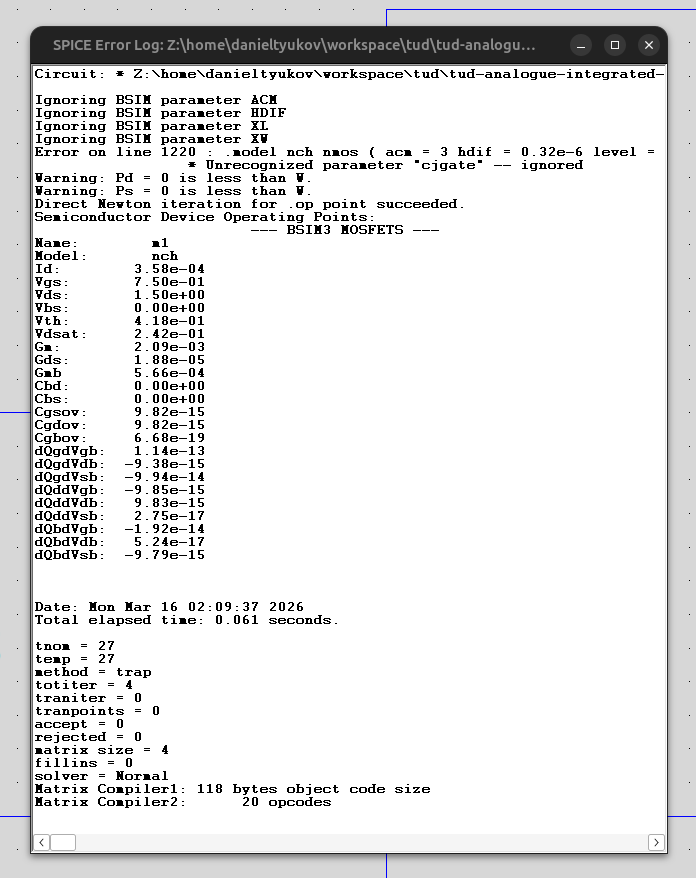
\includegraphics[width=0.75\textwidth]{imgs/partC_log_vgs0.75V.png}
\caption{SPICE error log showing BSIM3 operating point: $I_D = \SI{3.58e-4}{A}$, $g_m = \SI{2.09e-3}{S}$, $V_{th} = \SI{0.418}{V}$.}
\label{fig:partC_log}
\end{figure}

Simulation results: $I_D = \SI{357.7}{\micro A}$, $g_m = \SI{2.09}{mS}$, $V_{th} = \SI{0.418}{V}$.

\subsection{Error Analysis}

Percent error is calculated as:

\begin{equation}
\text{Error} = \frac{\text{estimate} - \text{ideal}}{\text{ideal}} \times 100\%
\end{equation}

where ``ideal'' refers to the LTSpice (BSIM3v3) value.

\begin{equation}
\text{Error}_{I_D} = \frac{243.6 - 357.7}{357.7} \times 100\% = -31.9\%
\end{equation}

\begin{equation}
\text{Error}_{g_m} = \frac{1.368 - 2.09}{2.09} \times 100\% = -34.5\%
\end{equation}

\subsection{Summary}

\begin{table}[H]
\centering
\caption{Square-law prediction vs.\ LTSpice simulation for $W/L = 20/0.7$, $V_{GS} = \SI{0.75}{V}$.}
\label{tab:partC}
\begin{tabular}{@{}lccc@{}}
\toprule
Parameter & Square-Law & LTSpice (BSIM3v3) & Error \\
\midrule
$I_D$ & \SI{243.6}{\micro A} & \SI{357.7}{\micro A} & $-31.9\%$ \\
$g_m$ & \SI{1.368}{mS} & \SI{2.09}{mS} & $-34.5\%$ \\
\bottomrule
\end{tabular}
\end{table}

\subsection{Conclusion}

The square-law model \textbf{significantly underestimates} both $I_D$ (by 32\%) and $g_m$ (by 35\%) for this device. The errors arise because:

\begin{enumerate}
\item \textbf{The extracted $V_t$ is wrong for this device.} The BSIM3v3 model gives $V_{th} = \SI{0.418}{V}$ at $L = \SI{0.7}{\micro m}$, while the square-law fit from $L = \SI{0.18}{\micro m}$ data yielded $V_t = \SI{0.394}{V}$. Threshold voltage is strongly $L$-dependent due to RSCE and SCE --- the square-law model has no mechanism to capture this.

\item \textbf{The extracted $\mu_n C_{ox}$ is wrong for this channel length.} Velocity saturation and mobility degradation are much less severe at $L = \SI{0.7}{\micro m}$ than at $L = \SI{0.18}{\micro m}$, so the effective mobility is higher than what was extracted --- the square-law underestimates the current.

\item \textbf{The square-law model itself is inadequate.} Even with correctly extracted parameters at this $L$, the quadratic $I_D$--$V_{GS}$ relationship does not accurately describe BSIM3v3 device behavior. This confirms the inapplicability of the square-law formula for \SI{180}{nm} MOS devices.
\end{enumerate}

%% ====================================================================
\section{Part D: Lookup Table Verification}
%% ====================================================================

Extract the same values from part~(c) using the lookup tables provided for the ET4252 technology. Show how they match the LTSpice simulation.

\subsection{Method}

The lookup tables (\texttt{180nch.mat}) contain pre-simulated BSIM3v3 data indexed by $(L,\, V_{GS},\, V_{DS},\, V_{SB})$. Using the \texttt{look\_up} function:

\begin{equation}
\frac{I_D}{W} = \texttt{look\_up}\!\left(\texttt{nch},\; \texttt{'ID\_W'},\; \texttt{'VGS'},\; 0.75,\; \texttt{'VDS'},\; 1.5,\; \texttt{'L'},\; 0.7\right)
\end{equation}

\begin{equation}
I_D = \frac{I_D}{W} \times W = 1.7846 \times 10^{-5} \times 20 = \SI{356.92}{\micro A}
\end{equation}

\begin{equation}
\frac{g_m}{I_D} = \texttt{look\_up}\!\left(\texttt{nch},\; \texttt{'GM\_ID'},\; \texttt{'VGS'},\; 0.75,\; \texttt{'VDS'},\; 1.5,\; \texttt{'L'},\; 0.7\right) = \SI{5.85}{S/A}
\end{equation}

\begin{equation}
g_m = \frac{g_m}{I_D} \times I_D = 5.85 \times 356.92 \times 10^{-6} = \SI{2.088}{mS}
\end{equation}

\subsection{MATLAB Script}

\begin{lstlisting}
load('180nch.mat');
VGS = 0.75; VDS = 1.5; L = 0.7; W = 20; % all in um

id_w  = look_up(nch, 'ID_W',  'VGS', VGS, 'VDS', VDS, 'L', L);
ID    = id_w * W;

gm_id = look_up(nch, 'GM_ID', 'VGS', VGS, 'VDS', VDS, 'L', L);
gm    = gm_id * ID;
\end{lstlisting}

\subsection{Results}

\begin{table}[H]
\centering
\caption{Lookup table results vs.\ LTSpice simulation for $W/L = 20/0.7$, $V_{GS} = \SI{0.75}{V}$.}
\label{tab:partD}
\begin{tabular}{@{}lccc@{}}
\toprule
Parameter & Lookup Table & LTSpice (BSIM3v3) & Error \\
\midrule
$I_D$ & \SI{356.92}{\micro A} & \SI{357.68}{\micro A} & $-0.21\%$ \\
$g_m$ & \SI{2.088}{mS} & \SI{2.09}{mS} & $-0.11\%$ \\
\bottomrule
\end{tabular}
\end{table}

The lookup table values match LTSpice to within $0.2\%$, confirming that the pre-computed tables accurately capture the BSIM3v3 device behavior.

\subsection{Full Comparison}

\begin{table}[H]
\centering
\caption{Complete comparison of all three methods for $W/L = 20/0.7$, $V_{GS} = \SI{0.75}{V}$, $V_{DS} = \SI{1.5}{V}$.}
\label{tab:full_comparison}
\begin{tabular}{@{}lcccc@{}}
\toprule
Method & $I_D$ & $g_m$ & $I_D$ Error & $g_m$ Error \\
\midrule
Square-law (Part C) & \SI{243.6}{\micro A} & \SI{1.368}{mS} & $-31.9\%$ & $-34.5\%$ \\
Lookup table (Part D) & \SI{356.92}{\micro A} & \SI{2.088}{mS} & $-0.21\%$ & $-0.11\%$ \\
LTSpice reference & \SI{357.68}{\micro A} & \SI{2.09}{mS} & --- & --- \\
\bottomrule
\end{tabular}
\end{table}

This confirms the inapplicability of the square-law formula and validates the $g_m/I_D$ lookup methodology as an accurate alternative for \SI{180}{nm} MOS device design.

\end{document}
